\usepackage{../pvm}

\usetikzlibrary{shadows,math}

\title{Technical Details}
\author{Fr\'ed\'eric Vogels}

\errorcontextlines 10000

\makeatletter
\pgfkeys{
  /ucll/pvm/.cd,
  start/.initial=0,
  size/.initial=1,
  height unit/.initial={0.75},
  contents/.initial={},
  id/.initial=sf,
  node style/.initial=unknown,
  stack frame/.style={minimum width=2cm,fill=red!50,font=\sc,draw},
  heap object/.style={minimum width=2cm,fill=blue!50,draw},
}
\newcommand{\alloc@block}[1][]{
  {
    \pgfkeys{
      /ucll/pvm/.cd,
      #1,
      /ucll/pvm/start/.get=\ucll@start,
      /ucll/pvm/size/.get=\ucll@size,
      /ucll/pvm/height unit/.get=\ucll@heightunit,
      /ucll/pvm/contents/.get=\ucll@contents,
      /ucll/pvm/node style/.get=\ucll@nodestyle,
      /ucll/pvm/id/.get=\ucll@id,
    }
    \tikzmath{
      real \ucll@y;
      real \ucll@height;
      \ucll@y = \ucll@start * \ucll@heightunit;
      \ucll@height = \ucll@size * \ucll@heightunit;
    }
    \node[\ucll@nodestyle,minimum height={\ucll@height cm},anchor=north west,font=\tiny] (\ucll@id) at (0,-\ucll@y) {\ucll@contents};
  }
}
\newcommand{\stackframe}[1][]{
  \alloc@block[node style=/ucll/pvm/stack frame,#1]
}
\newcommand{\heapobject}[1][]{
  \begin{scope}[xshift=2.3cm]
    \alloc@block[node style=/ucll/pvm/heap object,#1]
  \end{scope}
}

\newcommand{\memorylayout}{
  \node[anchor=south] at (1,0) {\textsc{stack}};
  \draw[fill=red!25] (-0.1,0.1) rectangle (2.1,-5.1);
  \begin{scope}[xshift=2.3cm]
    \node[anchor=south] at (1,0) {\textsc{heap}};
    \draw[fill=blue!25] (-0.1,0.1) rectangle (2.1,-5.1);
  \end{scope}
}
\makeatother

\begin{document}

\begin{frame}
  \titlepage
\end{frame}

\begin{frame}
  \frametitle{Call By Value}
  \code[frame=lines,width=.5\linewidth,font size=\small]{call-by-value.cpp}
  \begin{itemize}
    \item {\tt foo} receives a \emph{copy} of the passed object
    \item {\tt foo} knows the object's original values
    \item When {\tt foo} writes to {\tt b}, it writes to the copy
    \item {\tt foo} cannot write to the original object {\tt bar}
  \end{itemize}
\end{frame}

\begin{frame}
  \frametitle{Call By Value}
  \begin{center}
    \begin{columns}
      \column{4cm}
      \code[frame=lines,width=.95\linewidth,font size=\small]{call-by-value.cpp}
      \column{4cm}
      \begin{tikzpicture}
        \memorylayout

        \only<2->{
          \stackframe[start=0,contents={bar.x = 1}]
        }
        \only<3->{
          \stackframe[start=1,contents={bar.y = 2}]
        }
        \only<5-7>{
          \stackframe[start=2,contents={b.x = 2}]
        }
        \only<8-10>{
          \stackframe[start=2,contents={b.x = 3}]
        }
        \only<6-9>{
          \stackframe[start=3,contents={b.y = 3}]
        }
      \end{tikzpicture}
    \end{columns}
  \end{center}
  \vskip2mm
  \begin{overprint}
    \onslide<1-3>
    \begin{center}
      Creation of {\tt bar} on stack \\
      Default constructor is used
    \end{center}

    \onslide<4-6>
    \begin{center}
      Calling {\tt foo}: {\tt bar} is passed by value \\
      $\Rightarrow$ a copy is made \\
      $\Rightarrow$ copy constructor is called
    \end{center}

    \onslide<7-8>
    \begin{center}
      Incrementing {\tt b.x} operates on copy
    \end{center}

    \onslide<9-11>
    \begin{center}
      Returning from {\tt foo}: all locals are cleaned up \\
      $\Rightarrow$ {\tt b}'s destructor is called \\
    \end{center}

    \onslide<12>
    \begin{center}
      Note how {\tt bar} is still in its original state
    \end{center}
  \end{overprint}
\end{frame}


%%% Local Variables:
%%% mode: latex
%%% TeX-master: "technical-details"
%%% End:


% pass by value
% pass by pointer
% pass by reference
% return by value
% return by pointer
% return by reference
% operator = on T
% operator = on T*

\end{document}


%%% Local Variables:
%%% mode: latex
%%% TeX-master: "technical-details"
%%% End:
